\section{Implementación y pruebas}

% Introducción

\begin{frame}{Implementación}

Los componentes desarrollados se dividen en dos bloques:

\begin{itemize}[<+->]
\item \textbf{Módulo de telemetría.} Monitorizar el estado del sistema y enviar los paquetes al módulo de transmisión.
\item \textbf{Simulador térmico.} Control de la temperatura interna del sistema. Simulación software de componentes hardware.
\end{itemize}

\end{frame}

% Telemetría

\begin{frame}{Módulo de telemetría (1/2)}

\begin{figure}[h]
\centering
\resizebox{0.7\textwidth}{!}
{
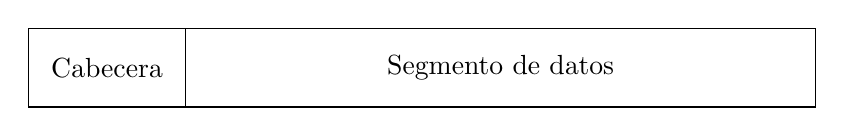
\begin{tikzpicture} 
 		\draw [black] (0,0) rectangle (10,1);
        \draw [black] (0,0) rectangle (2,1)node[pos=.5] (Header) {Cabecera};  
        \draw [black] (2,0) rectangle (10,1) node[pos=.5] (user) {Segmento de datos};       
        
\end{tikzpicture}
}
\caption{Estructura de paquete}
\end{figure}

\begin{itemize}
\item \textbf{Cabecera.} Identificador de paquete, \emph{checksum} y \emph{timestamp}.
\item \textbf{Segmento de datos.} Valores de sensores, actuadores y control del sistema.
\end{itemize}


Principales características:

\begin{itemize}
\item Evitar números en coma flotante (errores de precisión).
\item Reducir \emph{overhead} en sistemas empotrados.
\item Optimización de espacio empaquetando indicadores binarios en una variable de 32 bits.
\end{itemize}

\end{frame}


\begin{frame}{Módulo de telemetría (2/2)}

\begin{figure}
\centering
\resizebox{0.82\textwidth}{!}
{
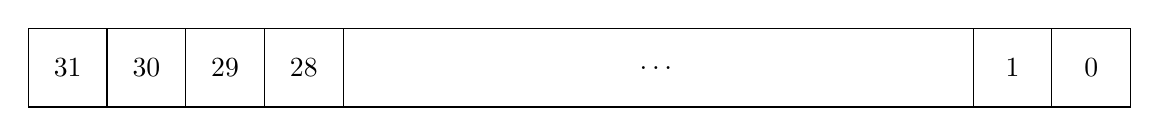
\begin{tikzpicture} 
 		\draw [black] (0,0) rectangle (14,1);
 		\draw [black] (0,0) rectangle (1,1)node[pos=.5] () {31};  
        \draw [black] (1,0) rectangle (2,1)node[pos=.5] () {30};  
         \draw [black] (2,0) rectangle (3,1)node[pos=.5] () {29};  
         \draw [black] (3,0) rectangle (4,1)node[pos=.5] () {28};  
          \draw [black] (4,0) rectangle (12,1)node[pos=.5] () {\ldots};  
           \draw [black] (12,0) rectangle (13,1)node[pos=.5] () {1};  
           \draw [black] (13,0) rectangle (14,1)node[pos=.5] () {0};  
             
        
       
\end{tikzpicture}
}
\caption{Empaquetado de indicadores binarios}
\end{figure}

\begin{columns}

\column{0.5\textwidth}

\begin{center}
\textbf{Paquete periódico}
\end{center}

\begin{itemize}
\item Envío periódico (0.2 Hz).
\item Toda la información del sistema.
\item Incluye \emph{flags} de estado.
\end{itemize}

\column{0.5\textwidth}

\begin{center}
\textbf{Paquete puntual}
\end{center}

\begin{itemize}
\item Envío $\Leftrightarrow$ solicitud del GS.
\item Diferentes tipos de paquetes (térmico, posicional y solar).
\item Incluye \emph{flags} de estado.
\end{itemize}

\end{columns}

\end{frame}


% Simulador térmico

\begin{frame}{Simulador térmico (1/2)}

Simulación software de los componentes térmicos del nanosatélite y módulo del OBSW.

\begin{itemize}[<+->]
\item \textbf{Calentadores.} Simulan un aumento de la temperatura.
\item \textbf{Termistores.} Simulan una lectura de temperatura.

\begin{center}
$T(t) = \mathcal{C} + A*sin(2\Pi\upsilon t + \varphi)$
\end{center}

\begin{figure}
\resizebox{0.8\textwidth}{!}{
 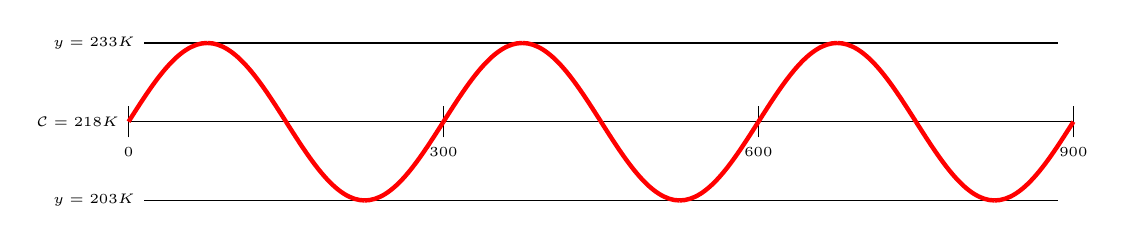
\begin{tikzpicture}
    \draw (0,0) -- (12,0);
    \draw (0.2,1)node[left,font=\tiny] {$y=233 K$} -- (11.8,1);
    \draw (0.2,-1)node[left,font=\tiny] {$y=203 K$} -- (11.8,-1); 
    \draw (0,0)node [left,font=\tiny,] {$\mathcal{C} = 218 K$};
    
    \draw (0,-0.2)node [below,font=\tiny,] {0} -- (0,0.2) ;
    \draw (4,-0.2)node [below,font=\tiny,] {300} -- (4,0.2) ;
    \draw (8,-0.2)node [below,font=\tiny,] {600} -- (8,0.2) ;
    \draw (12,-0.2)node [below,font=\tiny,] {900} -- (12,0.2) ;

    \draw[ultra thick, red] (0,0) sin (1,1);
    \draw[ultra thick, red] (1,1) cos (2,0);
    \draw[ultra thick, red] (2,0) sin (3,-1);
    \draw[ultra thick, red] (3,-1) cos (4,0);
    \draw[ultra thick, red] (4,0)  sin (5,1);
    \draw[ultra thick, red] (5,1) cos (6,0);
    \draw[ultra thick, red] (6,0) sin (7,-1);
    \draw[ultra thick, red] (7,-1) cos (8,0);
    \draw[ultra thick, red] (8,0) sin (9,1);
    \draw[ultra thick, red] (9,1) cos (10,0);
    \draw[ultra thick, red] (10,0) sin (11,-1);
    \draw[ultra thick, red] (11,-1) cos (12,0);
    \end{tikzpicture}
}  

\caption{Simulación lectura de temperatura}  
\end{figure}

\end{itemize}

\end{frame}


\begin{frame}{Simulador térmico (2/2)}

\begin{itemize}
\item \textbf{Control térmico.} Módulo de OBSW que controla la temperatura interna del sistema. 
\end{itemize}

Verifica los umbrales de temperatura de cada termistor y enciende/apaga su calentador asociado.

\begin{center}
$Termistor \rightarrow verificar$ $umbrales \rightarrow calentador$
\end{center}

Para lograr una simulación real, se añade un factor de ruido.

\begin{center}
$T_{i} = Thermistor_{i} + rand (-2,2) \mid \forall i \subset \{1,2,3\}$
\end{center}
 
\end{frame}


% Pruebas y evaluación

\begin{frame}{Pruebas y evaluación (1/2)}

Pruebas de verificación e integración para todos los componentes desarrollados.

\begin{columns}

\column{0.5\textwidth}

\begin{center}
\textbf{Entorno de pruebas}
\end{center}

\begin{itemize}
\item Intel Core i7 - 2.60 GHz.
\item 12 GB RAM DDR3.
\end{itemize}

\column{0.5\textwidth}

\begin{center}
\textbf{Sistema final}
\end{center}

\begin{itemize}
\item ARM Cortex A8 - 1 GHz.
\item 512 MB LPDDR RAM.
\end{itemize}

\end{columns}

\vspace{0.1 in}

Intervalo de confianza para comprobar que se cumplen las restricciones temporales.

\begin{figure}
$\mu = \bar{x}  \pm z {\sigma \over \sqrt{n}}$
\end{figure}

\end{frame}


\begin{frame}{Pruebas y evaluación (2/2)}

\begin{table}[h]
\centering
\resizebox{0.85\textwidth}{!}{
		\begin{tabular}{|c|c|c|c|}
		\hline 
		Módulo & Cómputo máximo (ms) & Cota inferior (ms) & Cota superior (ms)\\
		\hline
		Telemetría & 31.25 & 0.0168  & 0.0186 \\
		\hline
		Control térmico &  31.25 & 0.0162  & 0.0705\\	
		\hline
		\end{tabular}
		}
		\caption{Intervalo de confianza}
\end{table}

\begin{columns}

\column{0.5\textwidth}

\begin{figure}[h]
\centering
\includegraphics[width=0.98\textwidth]{rendimiento1}
\caption{Rendimiento telemetría}
\end{figure}

\column{0.5\textwidth}

\begin{figure}[h]
\centering
\includegraphics[width=\textwidth]{rendimiento2}
\caption{Rendimiento c. térmico}
\end{figure}

\end{columns}

\end{frame}